%%%%%%%%%%%%%%%%%%%%%%%%%%%%%%%%%%%%%%%%%%%%%%%%%%%%%%%%%%%%%%%%%%%%%%%%%%%%%%%%
% reconstruction.tex:
%%%%%%%%%%%%%%%%%%%%%%%%%%%%%%%%%%%%%%%%%%%%%%%%%%%%%%%%%%%%%%%%%%%%%%%%%%%%%%%%
\chapter{Data Analysis Strategy}
\label{Chapt:Data_Anaylysis_Stratagy}
\begin{chapquote}{ Douglas Adams, \textit{The Hitchhiker's Guide to the Galaxy }}
``Would it save you a lot of time if I just gave up and went mad now?"
\end{chapquote}
%%%%%%%%%%%%%%%%%%%%%%%%%%%%%%%%%%%%%%%%%%%%%%%%%%%%%%%%%%%%%%%%%%%%%%%%%%%%%%%%
We are measuring the Z boson  differential cross section in $\phistar$ and \rapidity. At its simplest, the observed differential cross section can be calculated as 
\begin{equation}
\label{eq:SimpleCross}
   \left[ \frac{ \dir \sigma}{\dir \phistar} \right]_i^{\mathrm{obs}}
   =
   \frac{N_i-B_i}{\luminosity \epsilon_i\Delta\phistar_i},
\end{equation}
where integrated luminosity is $\luminosity$, $\epsilon_i$ is the efficiency for reconstructing a Z in the bin given one was produced within the acceptance criteria,  $\Delta\phistar_i$ is the bin width, and $N_i$ and $B_i$ are the total number of Z candidates observed and the estimated background  in the $i$th bin respectively. Although the actual value of $B_i$ is unknown, since if we were able to count background events they would not be background, it can be estimated using simulation and data samples.

Equation \ref{eq:SimpleCross}  ignores bin migration, which happens when the kinematic properties of a lepton are reconstructed incorrectly which causes a event to be placed in the wrong \phistar bin. In the electron data set, this occurs for approximately 9.8\% of events. In order to find the ``true" \phistar distribution,\footnote{The \phistar distribution of the actual particles rather than the reconstructed ones} the measured distribution is corrected for bin migration or ``unfolded". This allows the data measurement to be compared to simulation which has a true, theoretical \phistar distribution. Because the simulation sample has both reconstructed events as well as generator level events the relationship between the two can be used to create a matrix $M_{ij}$ that allows for the true \phistar distribution of the data to be calculated based on the reconstructed values. This term can be used to create the final equation
\begin{equation}\label{eq:SlightlySimpleCross}
   \left[\frac{ \dir \sigma}{\dir \phistar}\right]_i^{\mathrm{unfold}}
   =
   \sum\limits_{j} M_{ij}\frac{N_j- B_j}{\luminosity \epsilon_j\Delta\phistar_j}.
\end{equation}
\section{Binning}
Due to a large change in differential cross-section of \phistar, it was chosen to not have uniform bin widths. Instead bin widths were chosen to have roughly the same number of events in each bin, except for the very high \phistar range. The boundaries of theses bins are given in Table \ref{table:phistarBins}
\begin{table}[!htbp]
\caption[\phistar bin ranges]{The range of \phistar bins.}
\label{table:phistarBins}
\begin{center}
\begin{tabular}{|c|c|c|c|}
\hline 
Bin \# & \phistar Range &Bin \# & \phistar Range \\ \hline 

 1 & 0.000-0.004 & 17 & 0.102-0.114  \\ \hline 
 2 & 0.004-0.008 & 18 & 0.114-0.145 \\ \hline 
 3 & 0.008-0.012 & 19 & 0.145-0.165 \\ \hline
 4 & 0.012-0.016 & 20 & 0.165-0.189 \\ \hline 
 5 & 0.016-0.020 & 21 & 0.189-0.219 \\ \hline 
 6 & 0.020-0.024 & 22 & 0.219-0.258\\ \hline  
 7 & 0.024-0.029 & 23 & 0.258-0.312\\ \hline 
 8 & 0.029-0.034 & 24 & 0.312-0.391\\ \hline
 9 & 0.034-0.039 &  25 & 0.391-0.524\\ \hline
 10 & 0.039-0.045 & 26 & 0.524-0.695\\ \hline
 11 & 0.045-0.052 & 27 & 0.695-0.918\\ \hline
 12 & 0.045-0.052 & 28 & 0.918-1.153\\ \hline
 13 & 0.052-0.057 & 29 & 1.153-1.496\\ \hline
 14 & 0.057-0.064 & 30 & 1.496-1.947\\ \hline
 15 & 0.081-0.091 & 31 & 1.947-2.522\\ \hline
 16 & 0.091-0.102 & 32 & 2.522-3.277\\ \hline


\end{tabular}
\end{center}

\end{table}


The boundaries for the rapidity bin were chosen to all be equal size of 0.4 and are shown in Table \ref{table:rapidity}. 

\begin{table}[!htbp]
\caption[\rapidity bin ranges]{The range of \rapidity bins.}
\label{table:rapidity}
\begin{center}
\begin{tabular}{|c|c|}
\hline 
Bin \# & \rapidity range \\ \hline
1 & 0.0-0.4 \\ \hline
2 & 0.4-0.8 \\ \hline
3 & 0.8-1.2 \\ \hline
4 & 1.2-1.6 \\ \hline
5 & 1.6-2.0 \\ \hline
6 & 2.0-2.4 \\ \hline
\end{tabular}
\end{center}
\end{table}
\section{Acceptance}\label{Sec:Acceptance}
A measurement such  as \phistar is subject to the limitation that not all electrons produced by  $\ensuremath{pp\to Z + X \to \ee + X}$ can be observed or triggered on by the CMS detector. As a result, the measurement can be reported in one of two ways. In the first option, we establish clear selections in simple kinematic variables. These selections are applied to both the data and the simulation samples before they are compared. The second method uses other simulation samples to attempt to calculate the full distribution of data based on the components that we are able to observe. This is then compared to the full distribution of a simulation sample. A disadvantage of the second method is that it is highly dependent on the simulation sample used and introduces additional sources of uncertainty. For this reason, the former method was chosen for this analysis.

Two acceptance selections required due to limitations of the detector, are selections on \pt and $\eta$ of the leptons. It is required that one lepton have $\pt > \SI{30}{GeV}$ and $|\eta| <2.1$, while the second lepton has looser requirements with $\pt > \SI{20}{GeV}$ and $|\eta| < 2.4$. The $\eta$ requirements were chosen to allow the use of the high-efficiency single-lepton triggers. Also, such events will be covered by both the ECAL and the tracker, allowing for a more precise angular measurement. The \pt bounds were chosen such that the leptons were not near the edge of the turn-on curve of the trigger.

\begin{figure}
    \centering
    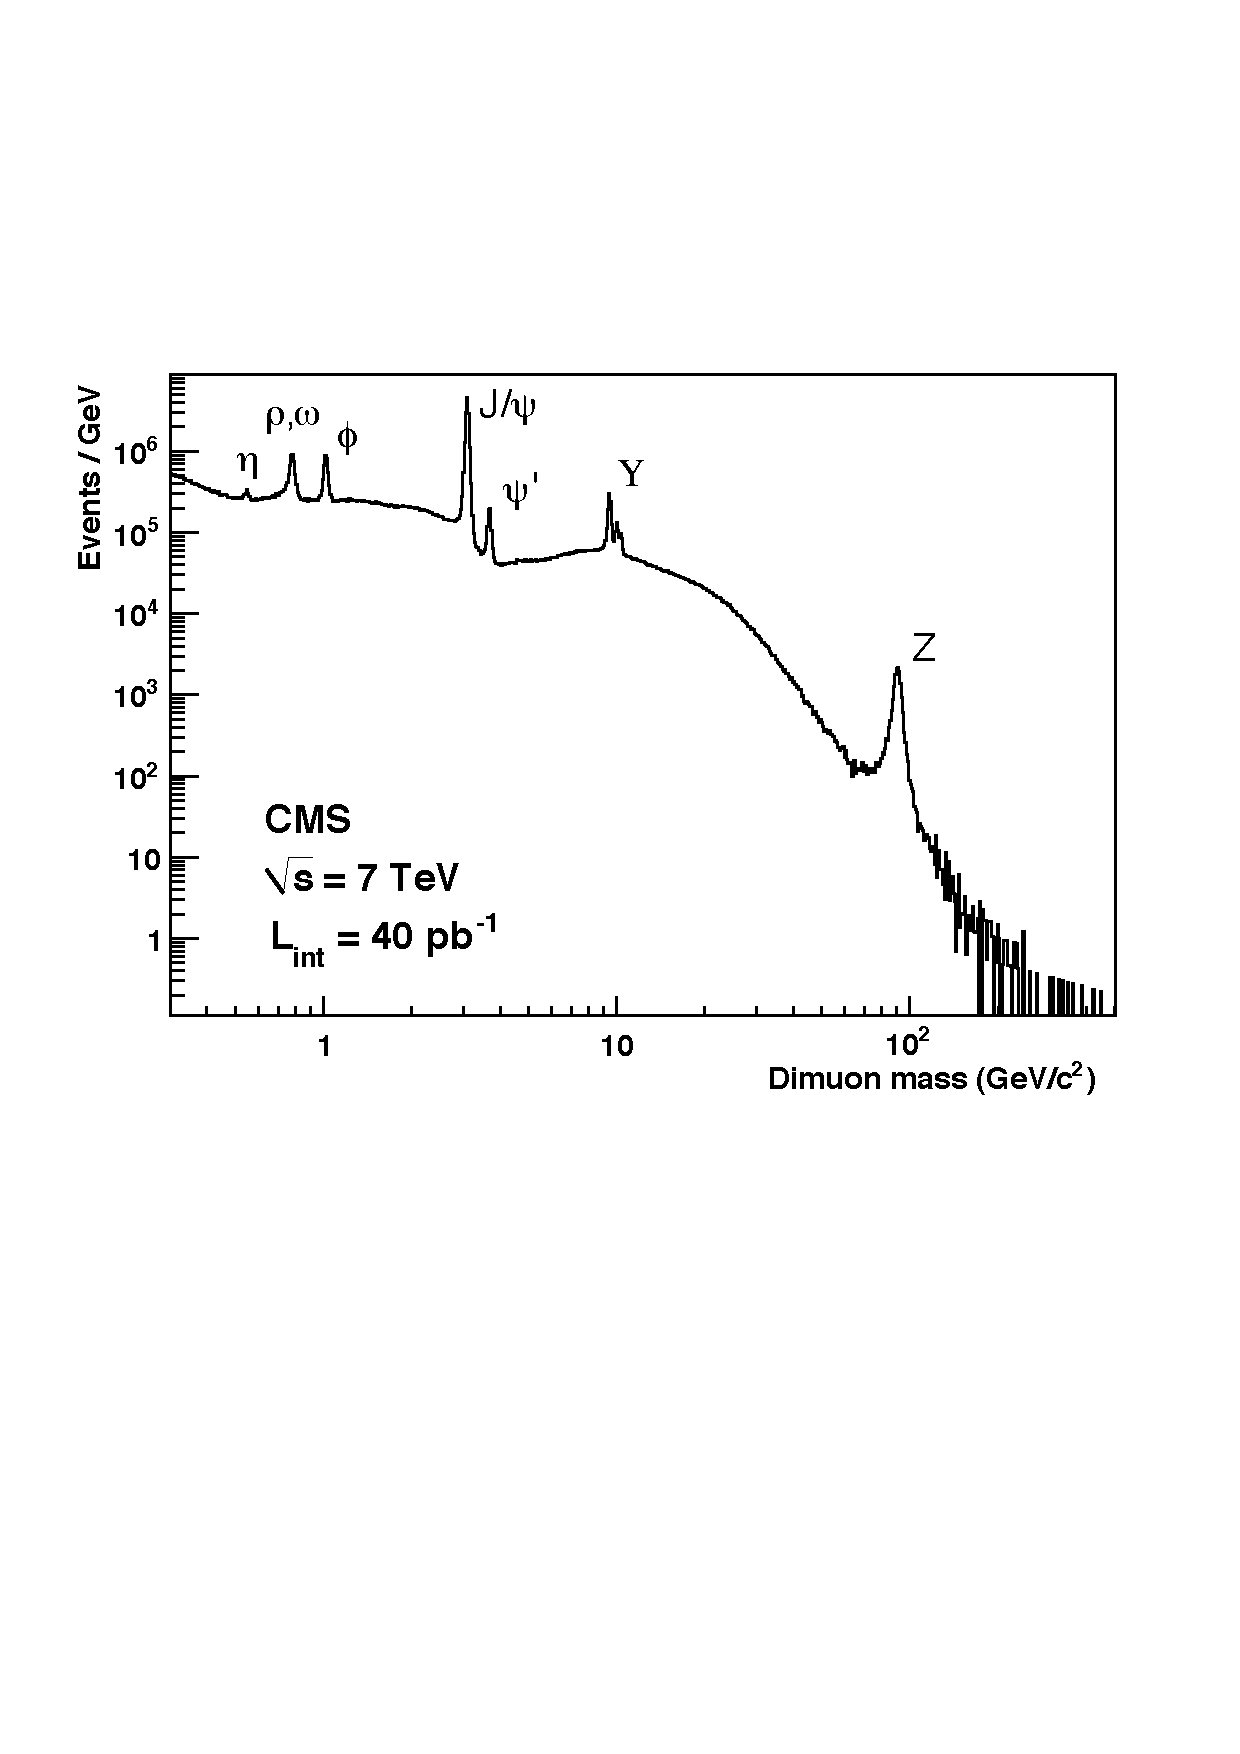
\includegraphics[width=\linewidth]{figures/DataAnaStrat/dimuonSpectrum_40pb-1.pdf}
    \caption{A distribution of the invariant mass of dimuon events at CMS 2010. Although many processes are capable of produce dileptons, almost all of them are produced with a invariant mass an order of magnitude smaller then the \Z.}
    \label{fig:DimuonMass}
\end{figure}
Another acceptance selection that is required is on the invariant mass of the lepton pair. As can be seen in Fig \ref{fig:DimuonMass}, many mesons are capable of producing a lepton pair, and there is a continuum distribution from virtual photons. To allow a precise interpretation of events arising from the initial hard-scatter, an acceptance selection on the mass is used to remove objects that decay to dileptons that were not a \Z by requiring $60<\mll<120$ GeV. 

The effect of the \pt and $\eta$ selections on the distribution of leptons can be seen in Fig \ref{fig:ElectronBeforeAfterCuts}, while the effects on the \Z mass and the \Z rapidity distributions can be seen in Fig \ref{fig:ZBosonBeforeAfterCuts}. All these distributions include the mass selection since further from the Z peak the photon component of the wave function becomes large compared to the \Z component.   

  \begin{figure}[!p]
    \centering
    \begin{subfigure}[b]{\SideBySidePlotWidth}
        \includegraphics[width=\linewidth]{figures/DataAnaStrat/AllElectEtaMCCompPlot.pdf}
        \caption{}
    \end{subfigure}%
    \begin{subfigure}[b]{\SideBySidePlotWidth}
        \includegraphics[width=\linewidth]{figures/DataAnaStrat/AllElectPtMCCompPlot.pdf}

    \end{subfigure}%

    \caption[
        ElectronsBefore and after acceptance 
    ]{
       These plots show the \pt and $\eta$ distribution of electrons that are produced from a Z decay. These results are from a simulated sample, showing the results of \pt and $\eta$ selections on the distribution. A invariant mass requirement of \MassRange was included with both distributions. Since different $\eta$ and \pt selections are used for the leading electron compared to the subleading electron a jump in the number of events can be seen in the after selections plots at $\eta=2.1$ and $\pt=30$.
    }
    \label{fig:ElectronBeforeAfterCuts}
\end{figure}

\begin{figure}[!p]
    \centering
    \begin{subfigure}[b]{\SideBySidePlotWidth}
        \includegraphics[width=\linewidth]{figures/DataAnaStrat/MassMCCompPlot.pdf}
        \caption{}
       % \label{fig:feyn_DYISR}
    \end{subfigure}%
    \begin{subfigure}[b]{\SideBySidePlotWidth}
        \includegraphics[width=\linewidth]{figures/DataAnaStrat/RapidityMCCompPlot.pdf}
        \caption{}
    \end{subfigure}%
    \hfill
      \caption[
        Higher order DY Feynman diagrams.
    ]{
       These plots show distribution of the mass of the \Z and its rapidity. These results are from a simulated sample, showing the results of \pt and $\eta$ selections on the distribution. Due to the \pt requirements on the electron, more massive Z bosons are likely to be kept, leading to an upward slope in the selection/total \MZ plot. The rapidity plot however is extremely flat up to where it quickly drops off at around $\rapidity=1$
    }
    \label{fig:ZBosonBeforeAfterCuts}
\end{figure}

    
    
  
\section{Efficiency, Background, and Unfolding}
The parameters, $\epsilon_i$ and $B_i$, which correspond to the efficiency and the background used in equations \ref{eq:SlightlySimpleCross}, are explored in depth in Chapters \ref{Chap:Efficiency} and \ref{data_set_chapter} respectively. The efficiency is the probability of a \Z whose properties pass acceptance being reconstructed. The backgrounds are events that can look like a $\Ztoee$ decay in our detector, and the unfolding is the matrix that corrects for bin migration.

\section{Unfolding}

Processing the data is pointless if there is nothing to compare it to. In theory we should be able to directly compare the data to a simulation sample. However due to detector effects, particles are never perfectly reconstructed, therefore the measured value of \phistar  can fall in a different bin from the real value. This is called bin migration. Fortunately, this bin migration is well modeled, since it is possible to simulate these detector effects and create a sample of reconstructed particles using the true particles. As can be seen in Fig \ref{fig:1DBinMigration}, which uses a \MADGRAPH sample, the majority of events' reconstructed and generated \phistar values fall in the same bin, however a non-trivial amount--about 9.8\%--fall in separate bins. Using this matrix it is possible to calculate the true distribution of the data using the reconstructed data, as well as the matrix shown in Fig \ref{fig:1DBinMigration}. 
\begin{figure}
    \centering
    \includegraphics[width=\linewidth]{figures/Simulation/GenRecoOneDTwoDPlot.pdf}
    \caption{A comparison of the Born vs reconstructed measured values. }
    \label{fig:1DBinMigration}
\end{figure}
\subsection{Two Dimensional Unfolding}
Although bin migration is relatively easy to represent for single measurements it becomes harder to represent when multiple measurements are done for each event. An example is a dual measurement of our Z samples where a measurement of both \phistar as well as the rapidity is made. Intuitively this would require a four-dimensional histogram, with two dimensions for both the generator and reconstructed values. This issue can be solved by representing higher dimensional studies as a larger 1D study. For the \phistar\rapidity study, this is done by having the first 36 bins represent all of \phistar measurement in which the rapidity of the \Z is $| \rapidity| <0.4$ , the next 36 bins represent all of \phistar measurement in which the rapidity of the \Z is $0.4<| \rapidity| <0.8$ and so on. These bins are shown in tables \ref{table:phistarAndEtaBins1} and \ref{table:phistarAndEtaBins2}. Using this method it is possible to represent two dimensions as a single axis. This allows us to represent the generated to  reconstructed measurements in a single 2D matrix shown in Fig. \ref{fig:2DBinMigration}.

\begin{table}[]
\begin{center}
\hspace*{-1.4cm}\begin{tabular}{|c|c|c|c|c|c|c|c|c|}
\hline 
Bin \# & \phistar Range &$\eta$  range & Bin \#  & \phistar Range &$\eta$  range & Bin \#& \phistar Range &$\eta$  range \\ \hline 

 1 & 0.000-0.004  & 0.0-0.4 & 33 & 0.000-0.004 & 0.4-0.8 & 65 & 0.000-0.004 & 0.8-1.2 \\ \hline
 2 & 0.004-0.008  & 0.0-0.4 & 34 & 0.004-0.008 & 0.4-0.8 & 66 & 0.004-0.008 & 0.8-1.2 \\ \hline
 3 & 0.008-0.012  & 0.0-0.4 & 35 & 0.008-0.012 & 0.4-0.8 & 67 & 0.008-0.012 & 0.8-1.2 \\ \hline
 4 & 0.012-0.016  & 0.0-0.4 & 36 & 0.012-0.016 & 0.4-0.8 & 68 & 0.012-0.016 & 0.8-1.2 \\ \hline
 5 & 0.016-0.020  & 0.0-0.4 & 37 & 0.016-0.020 & 0.4-0.8 & 69 & 0.016-0.020 & 0.8-1.2 \\ \hline
 6 & 0.020-0.024  & 0.0-0.4 & 38 & 0.020-0.024 & 0.4-0.8 & 70 & 0.020-0.024 & 0.8-1.2 \\ \hline
 7 & 0.024-0.029  & 0.0-0.4 & 39 & 0.024-0.029 & 0.4-0.8 & 71 & 0.024-0.029 & 0.8-1.2 \\ \hline
 8 & 0.029-0.034  & 0.0-0.4 & 40 & 0.029-0.034 & 0.4-0.8 & 72 & 0.029-0.034 & 0.8-1.2 \\ \hline
 9 & 0.034-0.039  & 0.0-0.4 & 41 & 0.034-0.039 & 0.4-0.8 & 73 & 0.034-0.039 & 0.8-1.2 \\ \hline
 10 & 0.039-0.045 & 0.0-0.4 & 42 & 0.039-0.045 & 0.4-0.8 & 74 & 0.039-0.045 & 0.8-1.2 \\ \hline
 11 & 0.045-0.052 & 0.0-0.4 & 43 & 0.045-0.052 & 0.4-0.8 & 75 & 0.045-0.052 & 0.8-1.2 \\ \hline
 12 & 0.045-0.052 & 0.0-0.4 & 44 & 0.045-0.052 & 0.4-0.8 & 76 & 0.045-0.052 & 0.8-1.2 \\ \hline
 13 & 0.052-0.057 & 0.0-0.4 & 45 & 0.052-0.057 & 0.4-0.8 & 77 & 0.052-0.057 & 0.8-1.2 \\ \hline
 14 & 0.057-0.064 & 0.0-0.4 & 46 & 0.057-0.064 & 0.4-0.8 & 78 & 0.057-0.064 & 0.8-1.2 \\ \hline
 15 & 0.081-0.091 & 0.0-0.4 & 47 & 0.081-0.091 & 0.4-0.8 & 79 & 0.081-0.091 & 0.8-1.2 \\ \hline
 16 & 0.091-0.102 & 0.0-0.4 & 48 & 0.091-0.102 & 0.4-0.8 & 80 & 0.091-0.102 & 0.8-1.2 \\ \hline
 17 & 0.102-0.114 & 0.0-0.4 & 49 & 0.102-0.114 & 0.4-0.8 & 81 & 0.102-0.114 & 0.8-1.2 \\ \hline
 18 & 0.114-0.145 & 0.0-0.4 & 50 & 0.114-0.145 & 0.4-0.8 & 82 & 0.114-0.145 & 0.8-1.2 \\ \hline
 19 & 0.145-0.165 & 0.0-0.4 & 51 & 0.145-0.165 & 0.4-0.8 & 83 & 0.145-0.165 & 0.8-1.2 \\ \hline
 20 & 0.165-0.189 & 0.0-0.4 & 52 & 0.165-0.189 & 0.4-0.8 & 84 & 0.165-0.189 & 0.8-1.2 \\ \hline
 21 & 0.189-0.219 & 0.0-0.4 & 53 & 0.189-0.219 & 0.4-0.8 & 85 & 0.189-0.219 & 0.8-1.2 \\ \hline
 22 & 0.219-0.258 & 0.0-0.4 & 54 & 0.219-0.258 & 0.4-0.8 & 86 & 0.219-0.258 & 0.8-1.2 \\ \hline
 23 & 0.258-0.312 & 0.0-0.4 & 55 & 0.258-0.312 & 0.4-0.8 & 87 & 0.258-0.312 & 0.8-1.2 \\ \hline
 24 & 0.312-0.391 & 0.0-0.4 & 56 & 0.312-0.391 & 0.4-0.8 & 88 & 0.312-0.391 & 0.8-1.2 \\ \hline
 25 & 0.391-0.524 & 0.0-0.4 & 57 & 0.391-0.524 & 0.4-0.8 & 89 & 0.391-0.524 & 0.8-1.2 \\ \hline
 26 & 0.524-0.695 & 0.0-0.4 & 58 & 0.524-0.695 & 0.4-0.8 & 90 & 0.524-0.695 & 0.8-1.2 \\ \hline
 27 & 0.695-0.918 & 0.0-0.4 & 59 & 0.695-0.918 & 0.4-0.8 & 91 & 0.695-0.918 & 0.8-1.2 \\ \hline
 28 & 0.918-1.153 & 0.0-0.4 & 60 & 0.918-1.153 & 0.4-0.8 & 92 & 0.918-1.153 & 0.8-1.2 \\ \hline
 29 & 1.153-1.496 & 0.0-0.4 & 61 & 1.153-1.496 & 0.4-0.8 & 93 & 1.153-1.496 & 0.8-1.2 \\ \hline
 30 & 1.496-1.947 & 0.0-0.4 & 62 & 1.496-1.947 & 0.4-0.8 & 94 & 1.496-1.947 & 0.8-1.2 \\ \hline
 31 & 1.947-2.522 & 0.0-0.4 & 63 & 1.947-2.522 & 0.4-0.8 & 95 & 1.947-2.522 & 0.8-1.2 \\ \hline
 32 & 2.522-3.277 & 0.0-0.4 & 64 & 2.522-3.277 & 0.4-0.8 & 96 & 2.522-3.277 & 0.8-1.2 \\ \hline



\end{tabular}

\end{center}
\caption[Half of the 2D bins ]{ The full list of unrolled \phistar,\rapidity bins for the double differential measurement. }
\label{table:phistarAndEtaBins1}
\end{table}


\begin{table}[!p]
\begin{center}
\hspace*{-1.4cm}\begin{tabular}{|c|c|c|c|c|c|c|c|c|}
\hline 
Bin \# & \phistar Range &$\eta$  range & Bin \#  & \phistar Range &$\eta$  range & Bin \#& \phistar Range &$\eta$  range \\ \hline 

97  & 0.000-0.004  & 1.2-1.6 & 129 & 0.000-0.004  & 1.6-2.0 & 161 & 0.000-0.004 & 2.0-2.4   \\ \hline 
98  & 0.004-0.008  & 1.2-1.6 & 130 & 0.004-0.008  & 1.6-2.0 & 162 & 0.004-0.008 & 2.0-2.4   \\ \hline 
99  & 0.008-0.012  & 1.2-1.6 & 131 & 0.008-0.012  & 1.6-2.0 & 163 & 0.008-0.012 & 2.0-2.4   \\ \hline
100 & 0.012-0.016  & 1.2-1.6 & 132 & 0.012-0.016  & 1.6-2.0 & 164 & 0.012-0.016 & 2.0-2.4   \\ \hline 
101 & 0.016-0.020  & 1.2-1.6 & 133 & 0.016-0.020  & 1.6-2.0 & 165 & 0.016-0.020 & 2.0-2.4   \\ \hline          
102 & 0.020-0.024  & 1.2-1.6 & 134 & 0.020-0.024  & 1.6-2.0 & 166 & 0.020-0.024 & 2.0-2.4   \\ \hline           
103 & 0.024-0.029  & 1.2-1.6 & 135 & 0.024-0.029  & 1.6-2.0 & 167 & 0.024-0.029 & 2.0-2.4   \\ \hline          
104 & 0.029-0.034  & 1.2-1.6 & 136 & 0.029-0.034  & 1.6-2.0 & 168 & 0.029-0.034 & 2.0-2.4   \\ \hline         
105 & 0.034-0.039  & 1.2-1.6 & 137 & 0.034-0.039  & 1.6-2.0 & 169 & 0.034-0.039 & 2.0-2.4   \\ \hline         
106 & 0.039-0.045  & 1.2-1.6 & 138 & 0.039-0.045  & 1.6-2.0 & 170 & 0.039-0.045 & 2.0-2.4   \\ \hline         
107 & 0.045-0.052  & 1.2-1.6 & 139 & 0.045-0.052  & 1.6-2.0 & 171 & 0.045-0.052 & 2.0-2.4   \\ \hline         
108 & 0.045-0.052  & 1.2-1.6 & 140 & 0.045-0.052  & 1.6-2.0 & 172 & 0.045-0.052 & 2.0-2.4   \\ \hline         
109 & 0.052-0.057  & 1.2-1.6 & 141 & 0.052-0.057  & 1.6-2.0 & 173 & 0.052-0.057 & 2.0-2.4   \\ \hline         
110 & 0.057-0.064  & 1.2-1.6 & 142 & 0.057-0.064  & 1.6-2.0 & 174 & 0.057-0.064 & 2.0-2.4   \\ \hline         
111 & 0.081-0.091  & 1.2-1.6 & 143 & 0.081-0.091  & 1.6-2.0 & 175 & 0.081-0.091 & 2.0-2.4   \\ \hline         
112 & 0.091-0.102  & 1.2-1.6 & 144 & 0.091-0.102  & 1.6-2.0 & 176 & 0.091-0.102 & 2.0-2.4   \\ \hline         
113 & 0.102-0.114  & 1.2-1.6 & 145 & 0.102-0.114  & 1.6-2.0 & 177 & 0.102-0.114 & 2.0-2.4   \\ \hline         
114 & 0.114-0.145  & 1.2-1.6 & 146 & 0.114-0.145  & 1.6-2.0 & 178 & 0.114-0.145 & 2.0-2.4   \\ \hline         
115 & 0.145-0.165  & 1.2-1.6 & 147 & 0.145-0.165  & 1.6-2.0 & 179 & 0.145-0.165 & 2.0-2.4   \\ \hline         
116 & 0.165-0.189  & 1.2-1.6 & 148 & 0.165-0.189  & 1.6-2.0 & 180 & 0.165-0.189 & 2.0-2.4   \\ \hline         
117 & 0.189-0.219  & 1.2-1.6 & 149 & 0.189-0.219  & 1.6-2.0 & 181 & 0.189-0.219 & 2.0-2.4   \\ \hline         
118 & 0.219-0.258  & 1.2-1.6 & 150 & 0.219-0.258  & 1.6-2.0 & 182 & 0.219-0.258 & 2.0-2.4   \\ \hline         
119 & 0.258-0.312  & 1.2-1.6 & 151 & 0.258-0.312  & 1.6-2.0 & 183 & 0.258-0.312 & 2.0-2.4   \\ \hline         
120 & 0.312-0.391  & 1.2-1.6 & 152 & 0.312-0.391  & 1.6-2.0 & 184 & 0.312-0.391 & 2.0-2.4   \\ \hline         
121 & 0.391-0.524  & 1.2-1.6 & 153 & 0.391-0.524  & 1.6-2.0 & 185 & 0.391-0.524 & 2.0-2.4   \\ \hline         
122 & 0.524-0.695  & 1.2-1.6 & 154 & 0.524-0.695  & 1.6-2.0 & 186 & 0.524-0.695 & 2.0-2.4   \\ \hline         
123 & 0.695-0.918  & 1.2-1.6 & 155 & 0.695-0.918  & 1.6-2.0 & 187 & 0.695-0.918 & 2.0-2.4   \\ \hline         
124 & 0.918-1.153  & 1.2-1.6 & 156 & 0.918-1.153  & 1.6-2.0 & 188 & 0.918-1.153 & 2.0-2.4   \\ \hline         
125 & 1.153-1.496  & 1.2-1.6 & 157 & 1.153-1.496  & 1.6-2.0 & 189 & 1.153-1.496 & 2.0-2.4   \\ \hline         
126 & 1.496-1.947  & 1.2-1.6 & 158 & 1.496-1.947  & 1.6-2.0 & 190 & 1.496-1.947 & 2.0-2.4   \\ \hline         
127 & 1.947-2.522  & 1.2-1.6 & 159 & 1.947-2.522  & 1.6-2.0 & 191 & 1.947-2.522 & 2.0-2.4   \\ \hline
128 & 2.522-3.277  & 1.2-1.6 & 160 & 2.522-3.277  & 1.6-2.0 & 192 & 2.522-3.277 & 2.0-2.4   \\ \hline



\end{tabular}
\end{center}
\caption[Other half of the 2D bin definitions]{The full list of unrolled \phistar,\rapidity bins for the double differential measurement. (continued) }
\label{table:phistarAndEtaBins2}
\end{table}





\begin{figure}
    \centering
    \includegraphics[width=\linewidth]{figures/Simulation/GenRecoTwoDTwoDPlot.pdf}
    \caption[\rapidity and \phistar unfolding matrix]{A comparison of Generated VS Reconstructed values for double differential measurement. As expected , migreation is largest for adjacent bins in \phistar or \rapidity, which may not be adjacent in the matrix which produces the observed pattern.}
    \label{fig:2DBinMigration}
\end{figure}

%%%%%%%%%%%%%%%%%%%%%%%%%%%%%%%%%%%%%%%%%%%%%%%%%%%%%%%%%%%%%%%%%%%%%%%%%%%%%%%%



